% !TEX encoding = UTF-8 Unicode
% !TEX root = main_org.tex


\chapter{Introduction}

One of the main goals of relativistic heavy ion collision experiments is to discover the confinement state, which is often called $Quark- Gluon- Plasma$ (QGP). Study of the properties of QGP status, such as equation of state, temperature, order of the phase transition, transport coefficient, and chemical evolution leads to a deeper understanding of dominant physics of heavy ion collision experiments. In this chapter, the basic motivation of heavy ion collision experiments and the measurement of the azimuthal correlation are introduced. 


\section{Quantum Chromo Dynamics (QCD)}

$Quantum$ $chromodynamics$ (QCD) is a fundamental theory relating to strong interactions between the quarks and gluons. QCD was developed as an extension of quantum electrodynamics(QED) by the imposition of a local SU(3) symmetry in ``color" space. The color confinement refers to the fact that quarks and gluons cannot be isolated and therefore cannot be observed directly. Quarks are confined within colorless particles called hadrons. Mesons are composed of quarks and anti-quarks ($q\bar{q}$), and baryons are composed of three quarks ($qqq$ or $\bar{qqq}$). The Strong interaction is governed by 
\begin{equation}
	V(r) = - \frac{4}{3} \frac{\alpha_s}{r} + kr,
	\label{eq:Strong}
\end{equation}
Where $\alpha_s$ is the coupling strength, and $k$ is the string tension. The second term in Eq.\ref{eq:Strong} shows that as the distance increases the attractive force increases, this force prevents the isolation of quarks. Therefore, all quarks are confined within hadrons, and not one can be observed as a free quark in nature. For example, when the distance between a quark-antiquark pair in a meson is increased by inserting more and more energy in the system, at some point it becomes more energetically favorable to produce a new quark-antiquark pair from the vacuum, which will then with the original quark-antiquark pair combine and form two new mesons, preventing in turn the quarks and antiquarks from original meson to be deconfined and to be found isolated.

The most important difference between QCD and QED is that QCD is a non-Abelian gauge theory and self-interacts with gluon as a consequence. The QCD interactions among quarks and gluons become weaker at high energy (called ``asymptotic freedom"), while the quarks and gluons are confined inside the hadrons at  low energy \cite{PhysRevLett.30.1346,PhysRevLett.30.1343}. The strong coupling constant $\alpha_s$ can be expressed as a function of the momentum transfer $Q^2$, as follows:

\begin{equation}
	\alpha_s(Q^2) \sim \frac{12\pi}{(33-2N_f)\ln(Q^2/\lambda^2_{QCD})}
\end{equation}
\bigskip

	where $N_f$ is the number of quarks flavors and $\lambda_{QCD} \sim 0.2$GeV is a typical QCD scale. When the momentum transfer $Q^2$ is large enough when compared with  $\lambda^2_{QCD}$, the $\alpha_s$ becomes small enough to allow the use of the perturbative method for QCD calculation (pQCD) as like in the QED \cite{PhysRevD.10.2445}. On the other hand, when $Q^2$ is not large enough, QCD remains in a  non-perturbative regime. 
	
		
	
\section {Quark Gloun Plasma (QGP)}

According to the ``Standard Model" quarks interact via a strong nuclear force which is carried by other elementary particles called gluons. The physical quantity for the strong interaction is $`color'$, which comes in three instances: red, blue and green, and the corresponding negative units(``anti-red'', ``anti-blue'', and ``anti-green''). Quarks carry only a single positive (negative) unit of color, while gluons carry the set of colors, i.e., they carry one positive and one negative unit of color. Since the strong interaction between quarks is transmitted via gluons, which carry only a discrete number of colors (gluons, for instance, do not have mass, charge, or flavor), the strong interaction only can change the color of the interacting quarks. For this reason the underlying fundamental theory of strong nuclear reaction is called ``$Quantum$ $Chromodynamics$" (QCD).

At ordinary temperatures and energy densities, normal matter is confined within a radius that corresponds to the QCD scale. However, at a sufficiently high temperature (or energy density), the color confinement can be broken. This phase transition from the confined nuclear matter to a deconfined state is the main subject of heavy ion collision physics. 

In relativistic heavy ion collision, the hadrons start to ``melt" into deconfined quarks and gluons. These transitions are predicted by Lattice QCD calculations \cite{Adams:2005dq} and produce Quark Gluon Plasma (QGP) as the state of matter consisiting of deconfined quarks and gluons (And Plasma is a general term used for physical system in which charges are screened due to the presence of other mobile charges). This QGP status is considered to have existed in the early universe, a few microseconds after the Big Bang \cite{PhysRevLett.34.1353, CABIBBO197567}. The Lattice QCD calculation predicts that the phase transition to a QGP state occurs at a critical temperature $T_c$ around $150\sim200$~MeV \cite{karsch}. This phase transition temperature might be reached in heavy-ion collisions currently delivered at RHIC with Au-Au collisions at a center of mass energy of 200~GeV per nucleon pair, and at LHC with Pb-Pb collision at a center of mass energy of 2.76~TeV per nucleon pair. The schematic phase diagram of QGP matter is illustrated in Fig.\ref{fig1}, where the horizontal axis is the baryon density and the vertical axis is the temperature. 
	
	
\begin{figure}[ht]
\centerline{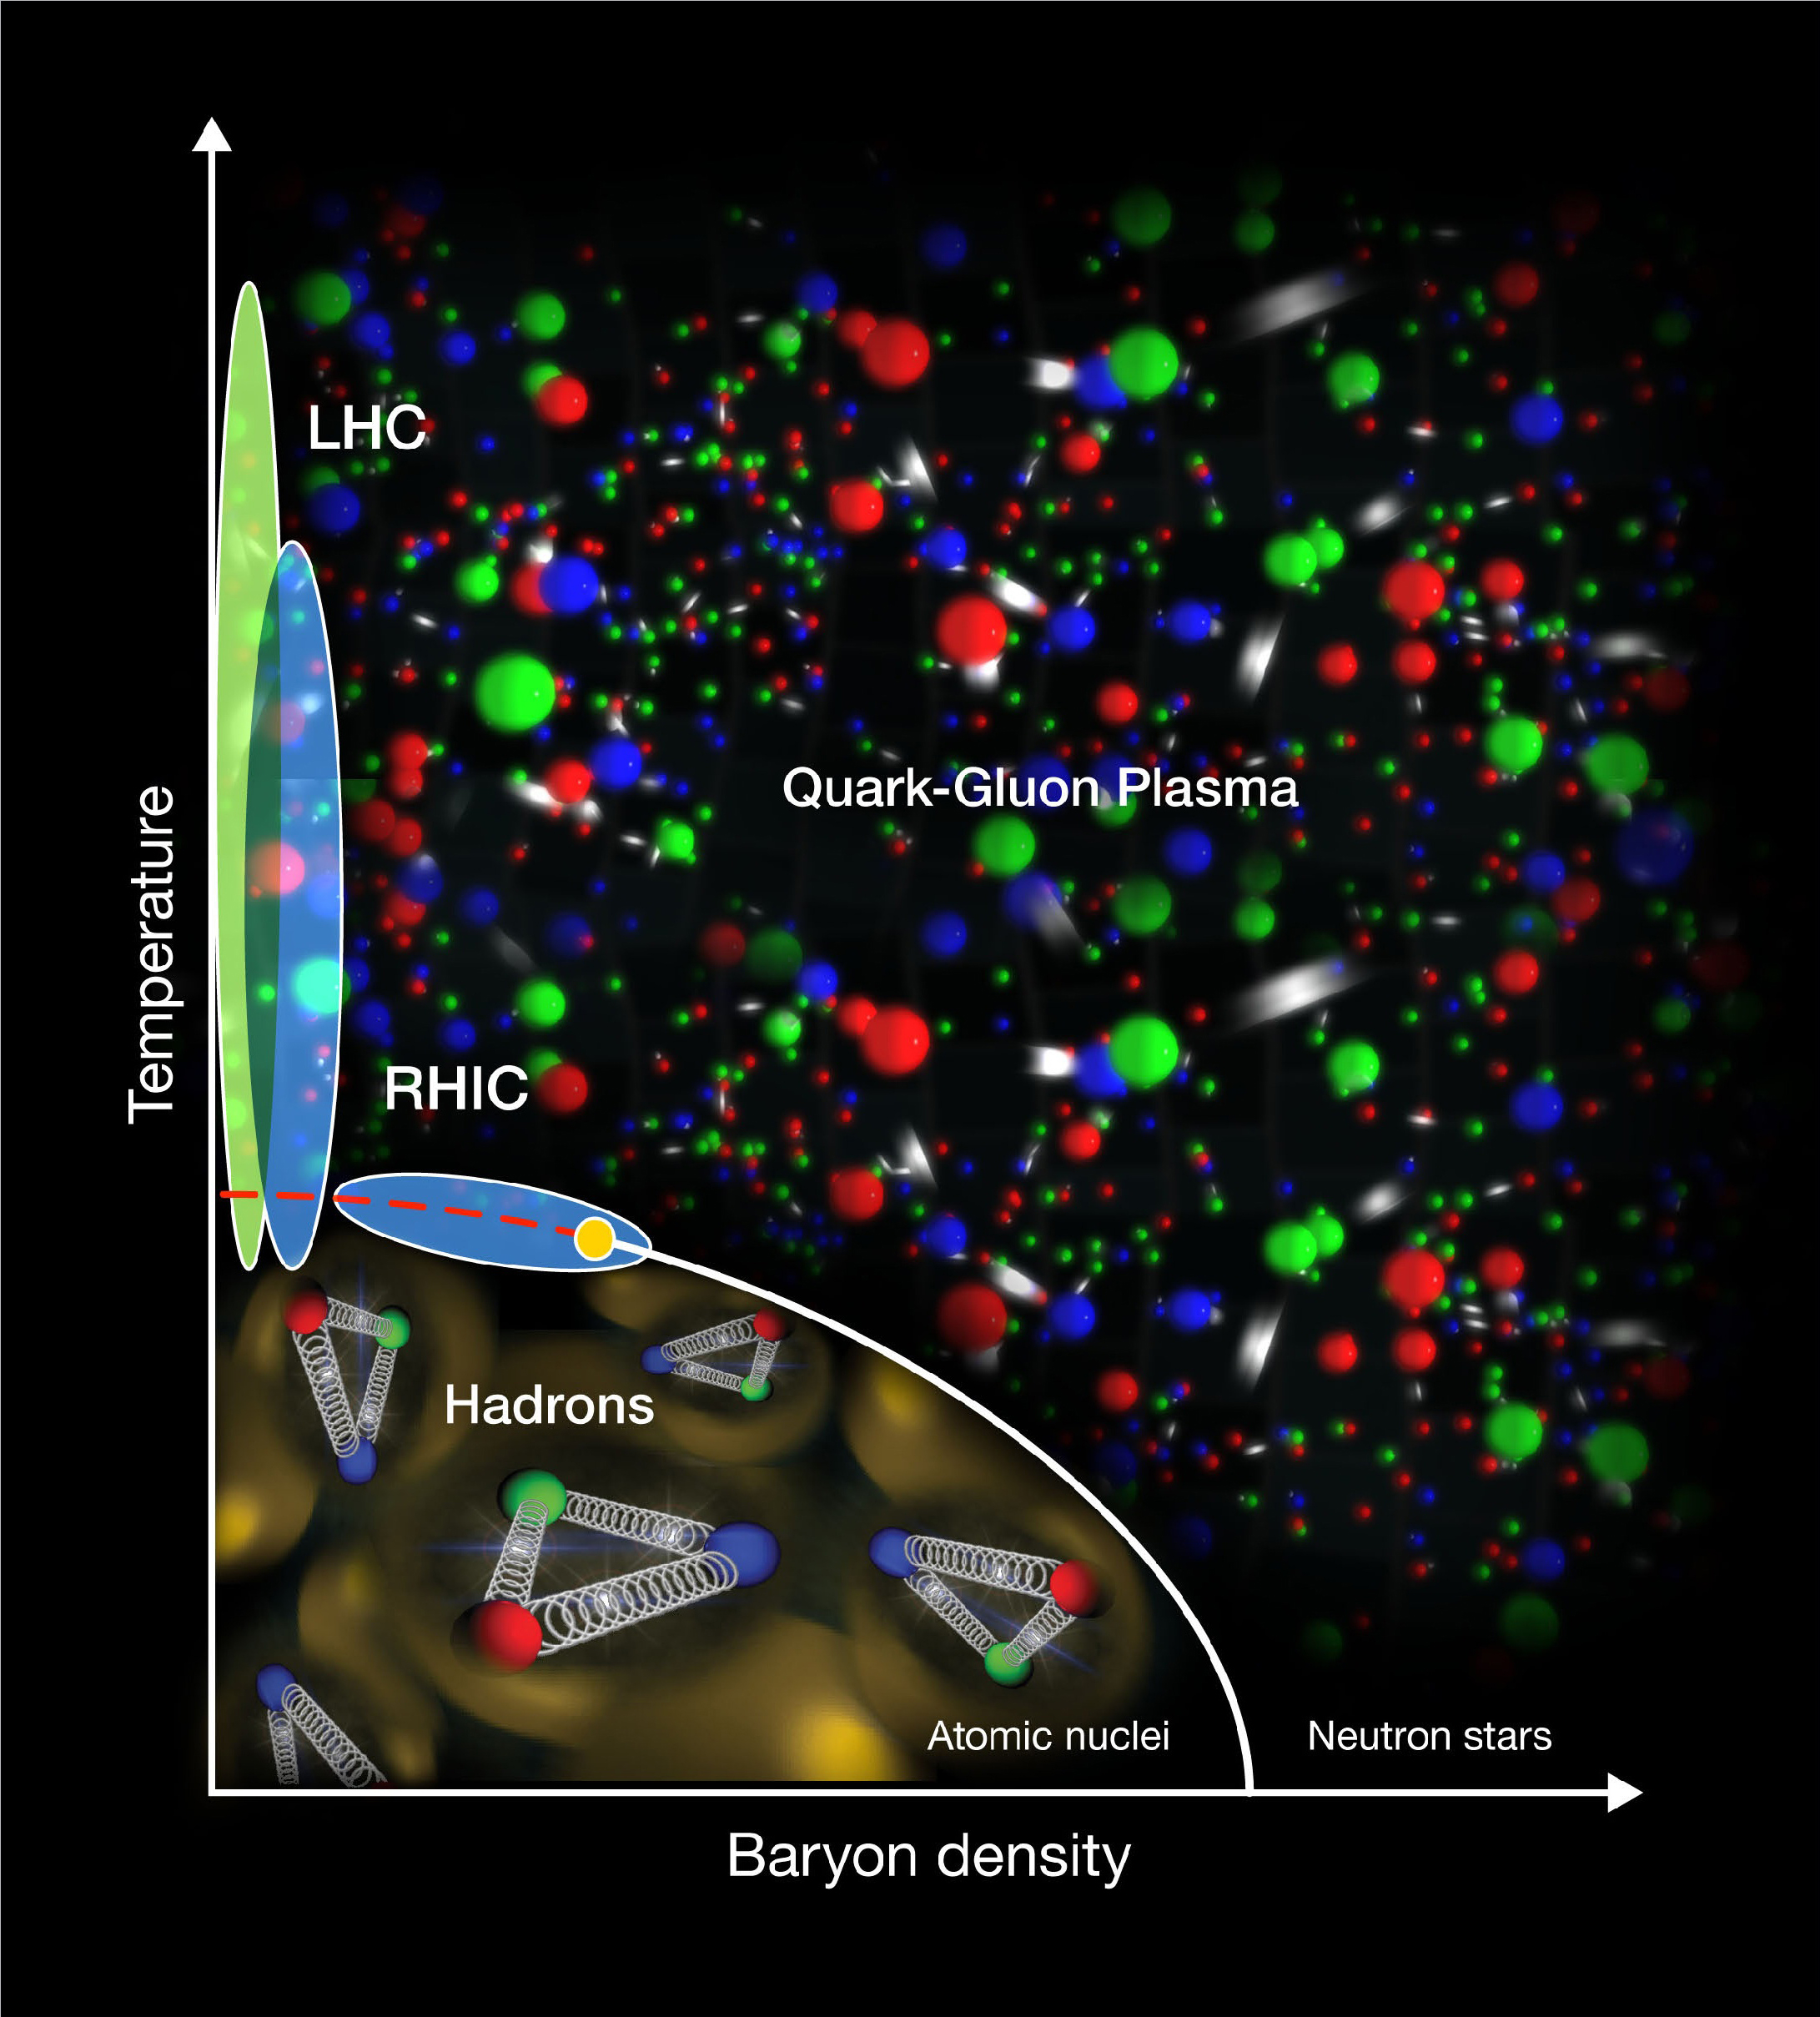
\includegraphics[width=10.0cm]{figures/RHIC_Graphics_Fig1-HR}}
\caption{A schematic phase diagram of QCD matter \cite{fig_phase_dia}}
\label{fig1}
\end{figure}



\section{Heavy ion collision}

As mentioned above, the universe started from a single point at approximately 14 billion years ago~(Big Bang), and expanded and cooled down. During this expansion, the transition from a QGP phase to a hadronic phase happened which allowed for the formation of hadrons.  To study this procedures, we collide heavy-ions at ultra-relativistic energies, where one creates QGP matter in the laboratory under controlled conditions. 

In the LHC experiment, the heavy ions are accelerated up to almost the speed of light and collide with each other. In this relativistic heavy ion collision, the initial energy density participating in the collision is expected to be well above the threshold for the QGP formation \cite{PhysRevD.27.140}.  In a canonical picture of the collision \cite{Kolb:2003dz} the system evolution can be divided into several stages, as shown in Fig.\ref{fig2}
  \begin{enumerate}
 	\item Initial state
 	\item thermalized QGP
 	\item hadronic gas
 	\item chemical freeze-out
 	\item kinetic freeze-out(free streaming)
 \end{enumerate}
 
 	At first, the two nuclei traveling at relativistic speeds become longitudinal Lorentz-contracted disks. A large number of the collisions between participants in target and projectile nuclei occur, and it is expected that the produced partons are strongly coupled with each other and thermalized into the QGP phase rapidly within a short time (less than a few fm/$c$). After $\sim 20$fm/$c$ the temperature of the expanding medium drops down below the critical temperature $T_c$ \cite{Rapp2011}. The quarks and gluons become confined into hadrons.  Afterward, the expansion (and the temperature fall) leads to a reduction of the inelastic processes among hadrons, until the relative abundance of hadron species is fixed (chemical freeze-out), and then to the stop of any interaction which fixes the kinetic spectra (kinetic freeze-out).
 	
 
\begin{figure}[h]
\centerline{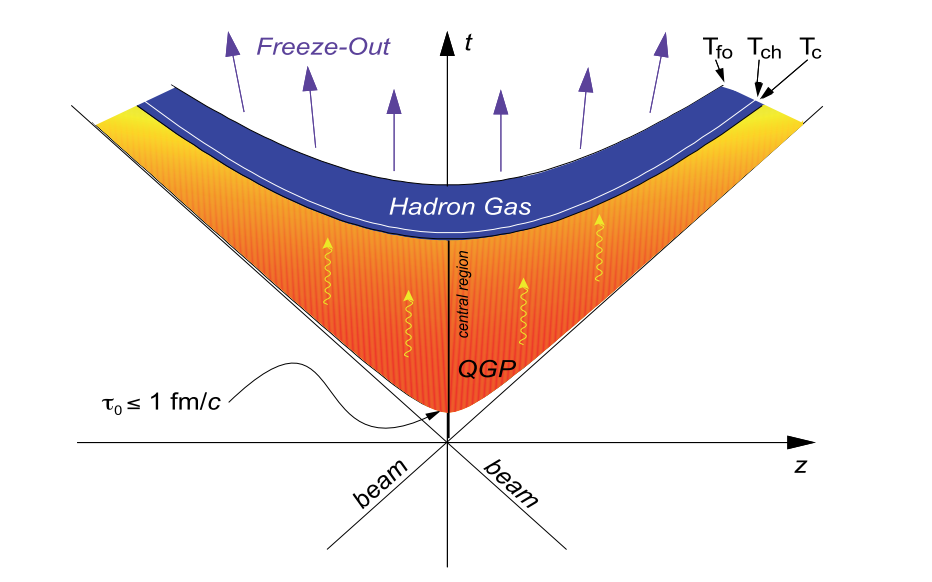
\includegraphics[width=13.0cm]{figures/system_evol}}
\caption{Schematic light cone diagram of the evolution of a high energy
heavy ion collision}
\label{fig2}
\end{figure}

	To verify the existence of the phase transition and the formation of QGP in heavy ion collisions, physics observables should be identified for each stage of dynamical evolution of the produced medium. Ordered in sequence of their formation in the course of the dynamics, the most relevant observables are characterized as follows:
	
	\begin{itemize}
		\item Suppression of heavy quarkonia production by Devye screening in the QGP
		\item Suppression of di-jets by losing their energy in the medium, so the undisturbed parton form a jet while the other one is absorbed in the medium and not detected (or distorted)
		\item High-$p_T$ particles produced in primordial $\hat{q}q, \hat{g}g, \hat{q}q$ reactions with high momentum transfer are attenuated by gluonic bremsstrahlung in QGP medium
		\item Hydrodanamics collective motion develops with the onset of thermal equilbrium
		\item Hadronic chemical freeze-out fixes the abundance ratios of the species
		\item Two particle Bose-Einstein-Correlations (the HBT effect of quantum optics) resulted from the kinetic freeze out stage
	\end{itemize}


 	Notably, the QGP matter collectively expand both in the longitudinal and the transverse direction. The transverse expansion leads the collectivity motion of system, which is often called the flow. The produced particles gain the momentum and energy from the radial flow of the QGP matter, and a final distribution of the transverse momentum is modified from the superposition of the independent nucleon-nucleon collisions \cite{Shen:2011eg}.
 	


\section{Flow}
\label{sec:flow}
\subsubsection{Introduction}
  In previous section, the phase transition is expected to occur at $T_c \sim 150$~MeV, corresponding to an energy density of $\epsilon_c \simeq 0.15 - 0.5$~GeV/$fm^3$ \cite{Bazavov:2014pvz}, which could be already be achieved at RHIC or LHC energies. Thus, experimental measurements in relativistic heavy ion collisions could shed light on the properties of the QGP. The main goal of studying relativistic heavy ion collisions is to discover and understand its properties of created matter. The system produced in relativistic heavy ion collisions dynamically evolves within a time duration of the order of fm/$c$. Therefore one has to describe the space-time evolution of thermodynamic variables to fill the large gap between the static aspects of QGP properties and the dynamical aspects of heavy ion collisions, and hydrodynamics plays an important role in connecting them. Hydrodynamics is thus applied to matter under local equilibrium in the intermediate stage.

Also by using hydrodynamics, we can remove QCD Lagrangian density

\begin{equation}
	\mathcal{L} = \bar{\psi_i}(i\gamma_\mu D^{\mu}_{ij} - m \delta_{ij})\psi_j - \frac{1}{4}F_{\mu v \alpha}F^{\mu v \alpha} 
\end{equation}
\smallskip

	where $\psi_i$ is a quark field, $\gamma$ are Dirac matrices, $D$ is a covariant derivative, $m$ is a quark mass, $\delta$ is the Kronecker delta symbol, and $F$ is the field strength of the gluons. In spite of simple looking of QCD Lagrangian form, it is very difficult to make any predictions directly from QCD due to its complexity which mainly arises from the non-linearity of the interactions of the gluons, the strong coupling, the dynamical many body system and confinement. In hydrodynamics, however, as a phenomenological theory, we can express the equation of state as follows: 
	
	\begin{equation}
		P = P(e, n)
	\end{equation}
	\smallskip 
	
	which expresses the pressure $P$ as a function of energy density $e$ and the baryon density $n$. Such an equation can be obtained by performing numerical simulations of QCD on the lattice. To calculate the above equation of the states, it is also necessary to use additional transport coefficients such as shear viscosity $\eta$, bulk viscosity $\zeta$, heat conductivity $\lambda$, etc. 
	
	%check it one more time
	Hydrodynamics can also produce outputs, such as local temperature or energy density, that could be useful in describing the dynamics for other observables. For instance, in the current formalism of jet quenching, one needs information regarding parton density or energy density along a trajectory of an energetic parton.
	
  Hydrodynamics also provides information regarding bulk matter. Therefore we can say that, in the context of relativistic heavy ion collisions, hydrodynamics is the heart of the dynamical modeling since it not only describes expansion and collective flow of matter, but also provides important information about the intermediate stage for other phenomena.
	
	\subsubsection{Formal definitions}
	The particle azimuthal distribution($r(\varphi$)) is a periodic quantity (over 0 to $2\pi$ in polar coordinate), and it can be expand with customary expressed in a Fourier series \cite{Voloshin:2008dg, Voloshin1996},
	
\begin{equation}
	r(\varphi)=\frac{x_0}{2\pi} + \frac{1}{\pi}\sum_{n=1}^{\infty}[x_n \cos(n\varphi) + y_n \sin(n\varphi)]
	\label{eq:flow}
\end{equation}
\smallskip
	
	
	where, Fourier coefficient $x_n, y_n$ is defined as
	
\begin{equation}
	x_n = \int_{0}^{2\pi} r(\varphi)\cos(n\varphi)d\varphi	
\end{equation}
\begin{equation}
	y_n = \int_{0}^{2\pi} r(\varphi)\sin(n\varphi)d\varphi	
\end{equation}
\smallskip

For our case, the multiplicity is finite, therefore $x_n$ and $y_n$ are changed into finite sum as like

\begin{equation}
x_n=\sum_{\nu}r_{\nu}\cos{n\phi_{\nu}}
\end{equation}
\begin{equation}
y_n=\sum_{\nu}r_{\nu}\sin{n\phi_{\nu}}
\label{eq:yndef}
\end{equation}
\smallskip

 $r_\nu$ is weight for particle, and usually it takes unity($r_v = 1$) for inclusive flow measurement. If there is no flow effect and fluctuation, the azimuthal distribution $r(\varphi)$ should be const. i.e. isotropic multiplicity for all angles, and all the coefficient of $\sin$ and $\cos$ terms will be vanished. On the other hand, if there are any anisotropic effect, coefficient $x_n$ and $y_n$ will survive. 
 
 If we define the $v_n$, and $\psi_n$ for each corresponding Fourier's harmonics in the following way:

\begin{equation}
	v_n \equiv \sqrt{x_n^2 + y_n^2}
\end{equation}
\begin{equation}
	0 \le \psi_n \le \frac{2\pi}{n} 
\end{equation}
\smallskip

we can now express azimuthal particle distribution with $v_n$ and $\psi_n$ instead of $x_n$ and $y_n$.

\begin{equation}
x_n=v_n \cos{n\psi_n}
\end{equation}
\begin{equation}
y_n=v_n \sin{n\psi_n}
\label{eq:xnyndef}
\end{equation}
\smallskip

If we put back $x_n$ and $y_n$ into original Eq.\ref{eq:flow}  then

\begin{equation}
\frac{dN}{d\phi}=\frac{x_0}{2\pi}+\frac{1}{\pi}\sum_{n=1}{(v_n\cos{n\psi_n}\cos{n\phi}+v_n\sin{n\psi_n}\sin{n\phi})}
\label{eq:flow_sinterm}
\end{equation}

\begin{equation}
=\frac{x_0}{2\pi}+\frac{1}{2\pi}\sum_{n=1}{(2v_n\cos{n(\phi-\psi_n)})}
\label{eq:flow_final}
\end{equation}
\smallskip


From Eq.\ref{eq:flow_sinterm} to \ref{eq:flow_final}, the sinus terms were vanished because of symmetry of the collision. As illustrated in Fig.\ref{fig3}, if the colliding nuclei are the same, the probability for a produced particles to be emitted in direction $\varphi$ and $-\varphi$ is equal. As defined in Eq.\ref{eq:yndef}, $y_n$ is average of $\langle \sin(n\varphi) \rangle$, and this average of sinus term will be canceled each other of any angle $\varphi$ with its symmetries
\begin{equation}
	\sin(n\varphi) + \sin(n(-\varphi)) = \sin(n\varphi) - \sin(n\varphi) =0
\end{equation}

From Eq.\ref{eq:flow_final}, harmonics $v_n$ can be related explicitly to the origin azimuthal distribution $r(\varphi)$ in the following way:

\begin{eqnarray}
	\langle \cos(n\varphi) \rangle &\equiv& \frac{\int_{0}^{2\pi}{\cos(n\varphi)r(\varphi)d\varphi}}{\int_0^{2\pi}{r(\varphi)d\varphi}} \\
	&=&\frac{\frac{1}{\pi} v_n \int_{0}^{2\pi}{\cos^2(n\varphi)d\varphi}}{v_0} \\ 
	&=& \frac{v_n}{v_0}
	\label{eq:vncal}
\end{eqnarray}

Using a normalized distribution $r( \varphi )$, for which $v_0 = \int_{0}^{2\pi}{r ( \varphi )} d\varphi = 1$, the above equation leads to:
	
\begin{equation}
	v_n = \langle \cos(n\varphi) \rangle 	
\end{equation}
\smallskip


	The harmonic $v_1$ is often called ``directed flow", and $v_2$ called ``elliptic flow", and $v_3$ is ``triangular flow". When we consider the polar coordinate with $(r, \varphi)$, then the distribution for eillipse-like is determined by the following equation. 
	

\begin{equation}
	r(\varphi) = \frac{a(1-\varepsilon^2)}{1+\varepsilon \cos \varphi}
\end{equation}
\smallskip

	where $\varepsilon$ is the eccentricity defined as 
\begin{equation}
	\varepsilon^2 \equiv 1 - \frac{b^2}{a^2}
\end{equation}

	with definition of a is major, and b is minor axis. With this parameterization, $v_n$ can be calculated analytically in a closed form, as like
\begin{equation}
	v_n = 2\pi b(-1)^{n}(\frac{a-b}{a+b})^{\frac{n}{2}}
\end{equation}

	The methods that attempt to explain the azimuthal distribution of particles produced with customized Fourier's expansion have been succeeded in relativistic heavy ion collision, especially in RHIC and LHC, by studying about strong collective and anisotropic flow in the transverse plane driven by the pressure gradients with more particles emitted in the direction of the largest gradients. The large elliptic flow discovered at RHIC energies \cite{Ackermann:2000tr} continuous to increase also in LHC energies \cite{Aamodt:2010pa,Adam:2016izf}. This has been predicted by calculations utilizing viscous hydrodynamics \cite{Romatschke:2007mq,Shen:2011eg,Schenke:2011zz,Bozek:2012qs,Gale:2012rq,Hirano:2010je}.

These calculations also demonstrated that the shear viscosity to the entropy density ratio ($\eta/s$) of strongly interacting matter is close to a universal lower bound $1/4\pi$ \cite{Kovtun:2004de} in heavy ion collisions at RHIC and LHC energies.

%The magnitude of the anisotropic flow has been to found to be sensitive to the transport properties, as well as the space-momentum profile in the initial state~\cite{}. 
The temperature dependence of the $\eta/s$ has some generic features that most of the known fluids obey. One such general behavior is that the ratio typically reaches its minimum value close to the phase transition region \cite{Lacey:2006bc}. 
It was shown, using kinetic theory and quantum mechanical considerations \cite{PhysRevD.31.53} that $\eta/s>1/15$ would be an order of magnitude for the lowest possible shear viscosity to entropy ratio in nature. Later it was found that one can calculate an exact lower bound $(\eta/s)_{\rm min}=1/4\pi\approx0.08$ using the AdS/CFT correspondence \cite{Kovtun:2004de}. Hydrodynamical simulations supports as well the view that the QGP matter indeed is close to that limit \cite{Gale:2012rq}. 	
	
	 In relativistic collision, each collision is characterized by the impact parameter, defined as the distance between the center of two nuclei points. Collisions with the short impact parameter are called central collisions and collisions with the long impact parameter are called peripheral collisions.  This geometry of the collision moments with non-central collision has ellipticity in the transverse plane and is shown in Fig.\ref{fig3}
	
\begin{figure}[t]
\centerline{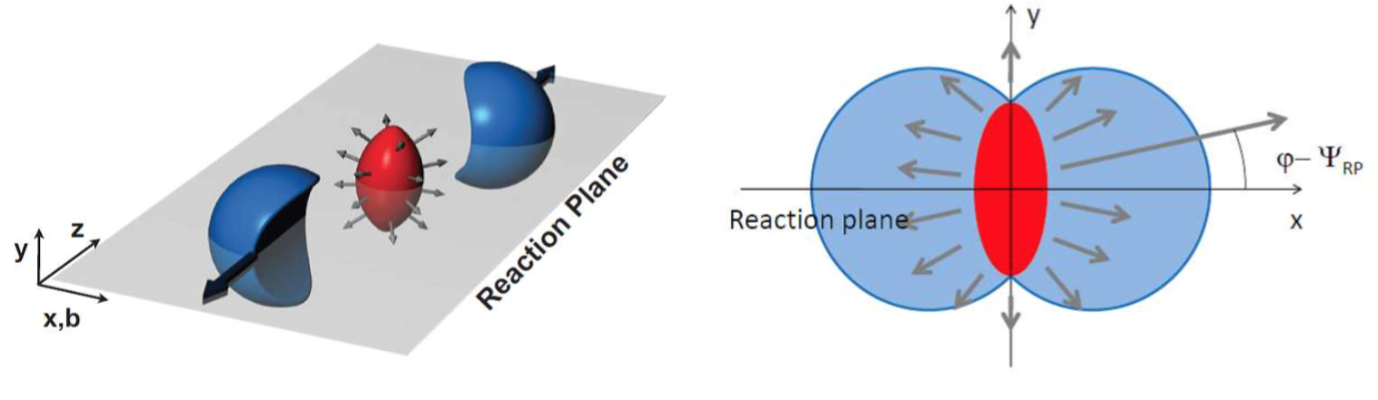
\includegraphics[width=13.0cm]{figures/flow_clasic}}
\caption{Schematic sketch of transverse projectile view of the non-central collision \cite{Snellings:2011sz}. The matter created in the collision (red) is called the participant region. The nucleons in the blue region are called spectators. The grey plane in the left figure is called the reaction plane.}
\label{fig3}
\end{figure}

	The initial spatial anisotropy in the azimuthal direction is transformed to the anisotropy of the final particle momentum distributions due to the collective expansion of the produced system. During evolution of the almond-shaped interaction volume, the anisotropy in coordinate space is transformed to anisotropy in momentum space (shown in Fig.\ref{fig4}). Therefore, these momentum anisotropies of the hydrodynamic matter lead to the anisotropic azimuthal distribution of the produced particles. 
	
	However, the transverse expansion of system volume is insufficient to explain the anisotropy of azimuthal particle distribution. As shown in Fig.\ref{fig5}, if there is no interaction between particles (or the mean free path among the produced particles is much longer than the typical size of the system), the azimuthal distribution of the particles does not depend on azimuthal angle on average due to symmetry of the production process. On the other hand, when the mean free path is very small compared to the typical system size, hydrodynamics can be applied to describe the space-time evolution of the system. Furthermore, the pressure gradient along the horizontal axis is much longer than the vertical axis due to the geometry.
 

 	
\begin{figure}[t]
\centerline{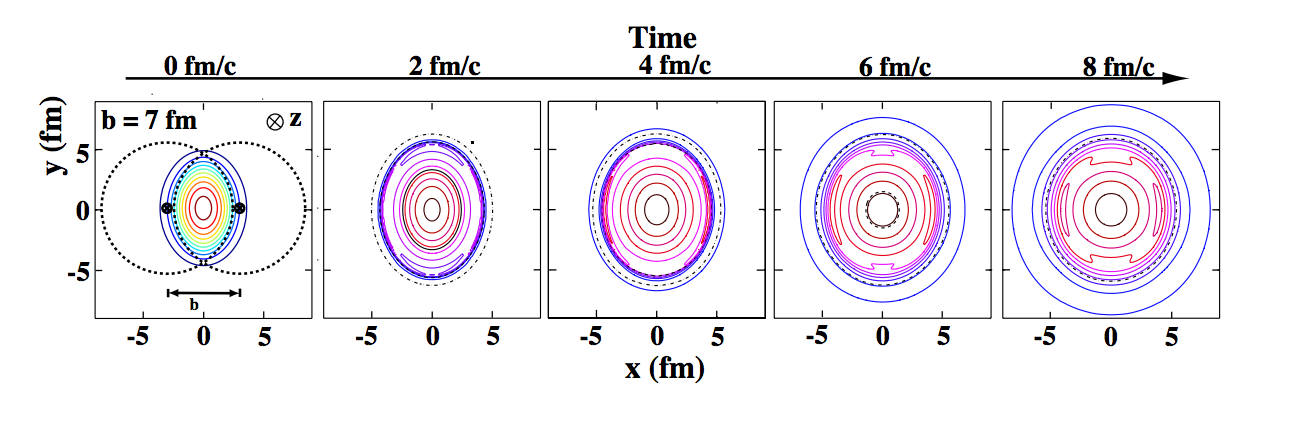
\includegraphics[width=12.0cm]{figures/system_time_flow}}
\centerline{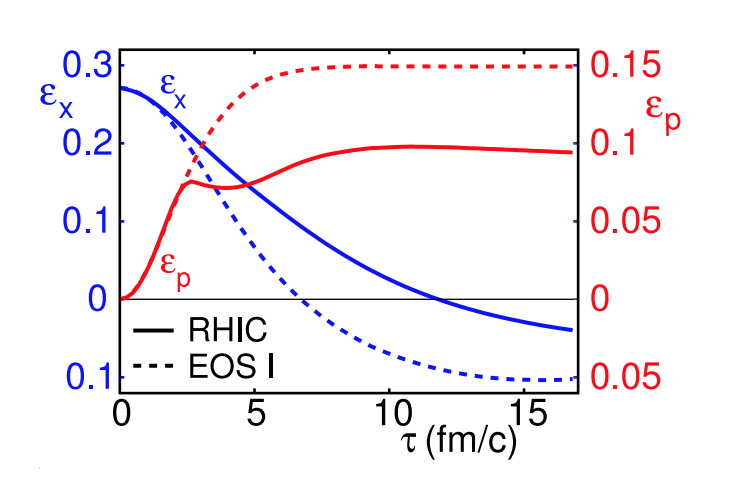
\includegraphics[width=9.0cm]{figures/time_ecenx_ecenp}}
\caption{The created initial transverse energy density profile and its time
dependence in coordinate space for a non-central heavy-ion collision \cite{Kolb:2003dz} As shown in the bottom figure, the anisotropy of space($\epsilon_x$) coordinate becomes smaller over time, while the momentum anisotropy of momentum space ($\epsilon_p$) increases as system expand as time goes. }
\label{fig4}
\end{figure}


	The origin of large $v_2$ cannot explain other harmonics especially odd number harmonics like $v_3$, $v_5$, etc. The impact parameter vector b (the vector connecting the centers of two colliding nucler) changes event-by-event, which in turn yields a random reaction plane angle $\psi_R$ (the plane spanned by the impact parameter and the beam axis). Due to these random fluctuations, it is not trivial to set up for each event the coordinate system. Because of the random geometry of participant nucleon in colliding nuclei, the overlap region shape is not a perfect almond shape, but rather a complex shape as shown in Fig.\ref{fig:complexshape}. As a result of this random fluctuation and the complex shape of the energy density profile of the system, the flow harmonics $v_n$ are defined with their own event plane $\psi_n$, not with respect to reaction plane $\psi_R$. Although the 2nd harmonics symmetry plane($\psi_2$) roughly corresponds to the reaction plane($\psi_2 \sim \psi_R)$, their azimuthal angles are slightly inclined event-by-event. In the following section, methods to calculate flow will be discussed.
		

\begin{figure}[h]
\centerline{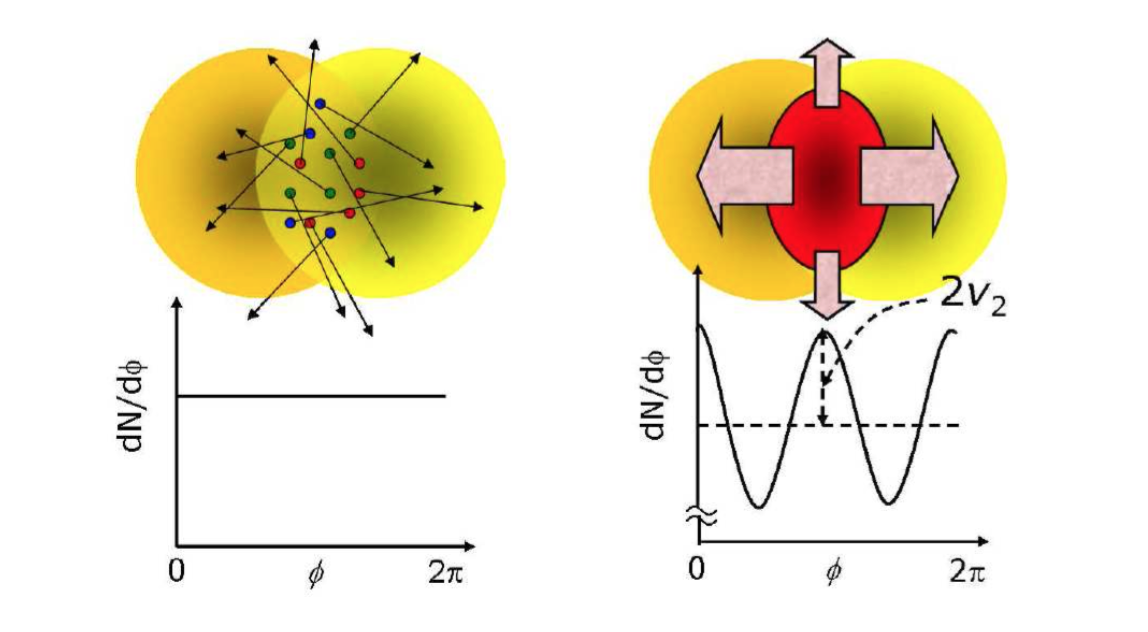
\includegraphics[width=13.0cm]{figures/v2explin}}
\caption{The illustration of the elliptic flow development in the two extreme cases: a large and small mean free path among the produced particles in the left and right images, respectively \cite{Voloshin:2008dg}.}
\label{fig5}
\end{figure}

\begin{figure}[h]
\centerline{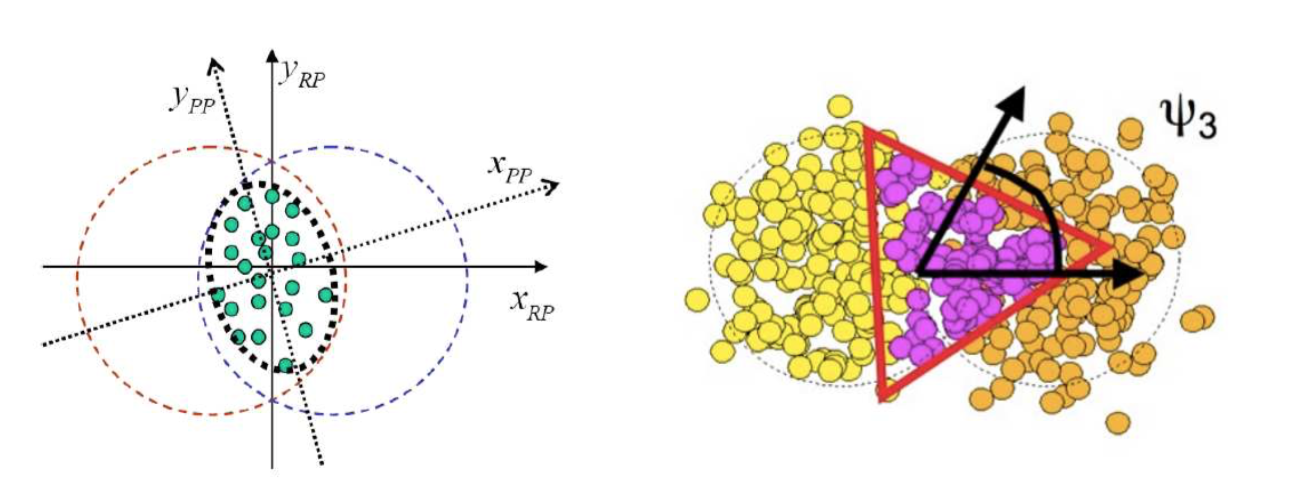
\includegraphics[width=13.0cm]{figures/fig_complxshape}}
\caption{The transverse profile in a single event simulated using the Monte Carlo Glauber model \cite{Miller:2007ri, Bzdak:2006qk}. (left) Green circles are the positions of the nucleon-nucleon collisions. The 2nd harmonic event plane is slightly inclined around the reaction plane. (right) It also has a non-zero triangle anisotropy. The azimuthal angle of the triangle anisotropy, i.e., the 3rd event plane angle $\Psi_3$ is not correlated to the reaction plane}
\label{fig:complexshape}
\end{figure}



\subsection{Event Plane method}

The event plane method (EP) is the most commonly used method to measure anisotropic flow. Using this method, the event plane is estimated and all particles' azimuthal angles are correlated to this estimated plane in order to obtain the flow harmonics $v_n$. From the Eq.\ref{eq:xnyndef} we can easily calculate event plane angles with the following way:


\begin{equation}
\frac{y_n}{x_n}=\frac{v_n\sin{n\psi_n}}{v_n\cos{n\psi_n}}=\tan{n\psi_n}
\end{equation}
\begin{equation}
\psi_n=(\arctan{\frac{y_n}{x_n}})/n
\end{equation}


and by using Fourier's coefficient relation:

\begin{equation}
v_n=\langle\cos{n(\phi_\nu - \psi_n)}\rangle 
\label{vndef}
\end{equation}
\smallskip


However, in practice, since each event has a finite number of created particles, the results for the event plane angle will be affected by a limited resolution. This can be corrected for by estimating the event plane resolution:

\begin{equation}
v_n^{measured}=\langle\cos{n({\phi-\psi_n^{measured})}}\rangle
\end{equation}
\smallskip

where, $\psi_n^{measured} = \psi_n + \psi_n^{err}$

\begin{eqnarray}
v_n^{measured}&=&\langle\cos{n(\phi-\psi_n-\psi_n^{err})}\rangle \\
&=&\langle\cos{n(\phi-\psi_n)}\cos{n(\psi_n^{err}})+\sin{n(\phi-\psi_n)}\sin{n(\psi_n^{err})}\rangle \\
&=&\langle\cos{n(\phi-\psi_n)}\cos{n(\psi_n^{err}})\rangle+\langle\sin{n(\phi-\psi_n)}\sin{n(\psi_n^{err})}\rangle \\
&=&\langle\cos{n(\phi-\psi_n)}\rangle\langle\cos{n(\psi_n^{err}})\rangle \\
&=&v_n\langle\cos{n(\psi_n^{err})}\rangle
\end{eqnarray}

Finally, we get 

\begin {equation}
v_n = v_n^{measured}/\langle\cos{n(\psi_n^{err})}\rangle
\end {equation}
\smallskip


We assume that event angle error($\psi_n^{err}$) is independent of $\phi-\psi_n$, and the expectation value of $\sin{n(\psi_n^{err})}$ is zero. The estimated event plane resolution can be obtained by two or more independent subevents \cite{PhysRevC.58.1671}. The advantage of the event plane method is that it is less sensitive to the number of particles for analysis, and can therefore be used to measure flow of rare particles. Furthermore, this method can be used to estimate an event plane, especially the 2nd order event plane which is expected to be similar to the reaction plane $\psi_2 \sim \psi_R$. This 2nd event plane also can be used for jet or other analysis. The main disadvantage of this method occurs when the event plane resolution is affected by correlations which do not stem from a genuine correlation of all particles with the true event plane. While event plane resolution can fix errors from multiplicity, it cannot fix errors originating from non-flow (e.g., jet, detector smearing, etc.). 

\subsection{Scalar product method}

	The original idea behind the event plane method is that the direction of $\Psi_n$ of the flow vector in a reference frame provides an estimation of the corresponding angle $\Phi_n$ in the underlying probability distribution. Because a finite sample of particles is used, statistical fluctuation causes $\Psi_n$ to differ from $\Phi_n$. This dispersion is characterized by the ``resolution", defined as
	
	\begin{eqnarray}
		R &\equiv & \langle e^{in(\Psi_n - \Phi_n} \rangle  \\
			&=& \left\langle \frac{Q_n}{|Q_n|} e^{-in\Phi_n} \right\rangle 
	\end{eqnarray}

	For the fixed $v_n$, the above equation can be written in the form of
	
	\begin{eqnarray}
		R(v_n) &\equiv &  \left\langle e^{in(\Psi_n - \Phi_n)} \right\rangle _{|vn} \\ 
		&=& \left\langle \frac{Q_n}{|Q_n|} e^{-in\Phi_n} \right\rangle _{|vn} \label{eq:res_def}
	\end{eqnarray}
	
	where $\langle ... \rangle _{|vn}$ indicates an average over a large number of event with the same underlying $v_n$. From the Eq.\ref{vndef}, we can see underlying probability distribution (Eq.\ref{eq:flow}) depends on the relative magnitude of the anisotropy $v_n$ to the statistical dispersion $1/\sqrt{N}$. In the limit $v_n \gg 1/\sqrt{N}$ (large number of multiplicity), easily reconstruct the underlying event plane so that $\Phi_n = \Psi_n$,(i.e. $R(v_n) \sim 1$, and conversely, when the $v_n \sqrt{N} \ll 1$ (low multiplicity) the Resolution $R(v_n) \sim kv_n$, where k is independent of $v_n$ and scale as $k \sim \sqrt{N}$. 
	
	%%% change this
	Generally, the value falls somewhere between these limits \cite{Luzum:2013yya}, and this nonlinear dependence of the resolution on the underlying flow is the origin of the difficulties of the event plane method.
	
	When we obtain the event plane resolution from subevents A and B, the resolution $R(v_n)$ is a factorization like the below  definition:
	
	\begin{eqnarray}
		\left \langle \frac{Q_{nA}}{|Q_{nA}|}  \frac{Q_{nB}}{|Q_{nB}|} \right \rangle &=&  \left \langle \frac{Q_{nA}}{|Q_{nA}|} e^{-in\Phi_n} \right \rangle \left \langle \frac{Q_{nB}}{|Q_{nB}|} e^{-in\Phi_n} \right \rangle^{*} \\
		&=& \left |   \left \langle   \frac{Q_{nA}}{|Q_{nA}|} e^{-in\Phi_n}  \right \rangle _{|v_n} \right | ^{2} \\ 
		&=&  R(v_{nA})^2
	\end{eqnarray}
	The Eq.\ref{eq:res_def} is used for the second line to third line of the above equation. The event-plane methods is thus defined as:
	
	\begin{equation}
		v_n\{EP\} \equiv \frac{\left \langle Q_n \frac{Q_{nA}^*}{|Q_{nA}|} \right \rangle }{\sqrt{\left \langle  \frac{Q_{nA}}{|Q_{nA}|}  \frac{Q_{nB}}{|Q_{nB}|} \right \rangle }}
		\label{eq:EP}
	\end{equation}
	\smallskip
	
	Since the measurement has been taken with the average of all events in a given centrality class, Eq.\ref{eq:EP} changes as term of $v_n$ as like
	
	\begin{equation}
		v_n\{EP\} = \frac{\langle v_n R(v_{nA})\rangle _{v_n}}{\sqrt{\langle R(v_{nA})^2 \rangle _{v_n} }}
	\end{equation}
	\smallskip 
	
	Note that $\langle R(v_{nA})^2 \rangle \neq \langle R(v_{nA})\rangle ^2$. Resolution correction is no longer a simple projection of the measured event plane $\Psi_n$ onto the ``true" event plane $\Phi_n$.
	
	In the limit of infinite multiplicity (i.e. $R(v_n) \sim 1$), $v_n\{EP\}$ does indeed measure the event averaged mean $v_n$ from Eq.\ref{eq:flow}. But in reality, the resolution is not perfect and the result is usually even closer to the low resolution limit \cite{Alver:2008zza}, and in this case, the event-plane measurement thus yields a root-mean-square value. In other words, what we measure with the event plane method is some values between root-mean-square and mean of $v_n$ depends on the resolution (i.e. Event multiplicity or the performance and acceptance of detector)
	
	\begin{equation}
		v_n\{EP\} \simeq \langle v_n \rangle \quad \text{(high resolution limit)}
	\end{equation}

	\begin{equation}
		v_n\{EP\} \simeq \sqrt{\langle v_n^2 \rangle}  \quad \text{(low resolution limit)}
	\end{equation}
	\smallskip
	
	However, in the scalar product method, which is a slight variant of the event plane method, consists of removing the factor of $|Q_n|$ before taking the average in the numerator and denominator of Eq.\ref{eq:EP}
	
	
	\begin{equation}
		v_n\{SP\} \equiv \frac{\langle Q_n Q_{nA}^*\rangle}{\sqrt{\langle Q_n Q_{nA}^*\rangle}}
	\end{equation}
	\smallskip 
	
		Then, by calculating the scalar product in numerator, the fluctuation term (Resolution related terms) are removed. 
		
	\begin{equation}
		v_n\{SP\} = \frac{\langle v_n v_{nA} \rangle _{v_n} }{\sqrt{\langle v_n v_{nA} \rangle _{v_n}}} = \sqrt{\langle v_n^2 \rangle }
	\end{equation}	
	\smallskip
	
	As a result, the scalar product method always yields the root-mean-square $v_n$, regardless of the details of the analysis and makes for a superior measurement. 
	
\subsection{Cumulants method}

\subsubsection{Multi particle correlations}

Because of the disadvantage of the event plane method (or the scalar product method) in estimating the event plane, the cumulants method (often called the multi-particle correlation method) was proposed in order to reduce this bias. This method does not require the event plane estimation event-by-event. Instead, these multi-particle correlations can be calculated by looping over all possible multiplets. If we assume that all the particles have azimuthal correlations which originated from flow harmonics only, then 2- and 4- particle azimuthal correlations can be expressed in the following way:
	
\begin{equation}
	\langle 2 \rangle \equiv  \langle e^{in(\phi_1 - \phi_2)} \rangle \equiv \frac{1}{{M \choose 2}2!}\sum_{i,j=1, i\neq j}^{M}{e^{in(\phi_i - \phi_j)}}
\end{equation}
\begin{equation}
	\langle 4 \rangle \equiv \langle e^{in(\phi_1 + \phi_2 - \phi_3 - \phi_4} \rangle \equiv \frac{1}{{M \choose 4}4!}\sum^{M}_{i\neq j\neq k \neq l}e^{in(\phi_i + \phi_j - \phi_k - \phi_l)}
\end{equation}
\smallskip

where the brackets denote the particle average in a single event. The $i, j, k, l$ denote identical particles, and $\phi_i$ is the azimuthal angle of the $i$-th particle measured in laboratory frame. To prevent contribution of self(auto) correlation, the constraints $i \neq j$ and $i \neq j \neq k \neq l$ have been enforced. When we extend the above equation for event average, then 2- and 4- particle azimuthal correlations are as follows :

\begin{equation}
	\langle \langle 2 \rangle \rangle \equiv \langle \langle e^{in(\phi_1 - \phi2)} \rangle \rangle \equiv \frac{\sum_{i=1}^{N}{(W_{\langle 2 \rangle})_i}\langle 2 \rangle_2 }{\sum_{i=1}^{N}{(W_{\langle 2 \rangle})_i}}
\end{equation}
\begin{equation}
	\langle \langle 4 \rangle \rangle \equiv \langle \langle e^{in(\phi_1 + \phi_2 - \phi_3 - \phi_4)} \rangle \equiv \frac{\sum_{i=1}^{N}{(W_{\langle 4 \rangle })_i}\langle 4 \rangle_i }{\sum_{i=1}^{N}{(W_{\langle 4 \rangle})_i}}
\end{equation}
\smallskip

where, N is the number of events, and $W_{\langle 2 \rangle}$ and $W_{\langle 4 \rangle}$ are the event weights. The selecting event weight is explained in Appendix B. The benefit of using multi-particle azimuthal correlation is to measure flow harmonics $v_n$ without requiring the event plane $\psi_n$, 

\begin{eqnarray}
	\langle \langle 2 \rangle \rangle \equiv \langle \langle e^{in(\phi_1 - \phi_2)} \rangle  \rangle &=& \langle \langle e^{in(\phi_1 - \psi_n - \phi_2 + \psi_n)} \rangle \rangle  \\
		&=& \langle \langle e^{in(\phi_1 - \psi_n)} \rangle \langle e^{-in(\phi_2-\psi_n)} \rangle \rangle = \langle v_n^2 \rangle
		\label{eq:vn2}
\end{eqnarray}

In cases when only flow correlations exist in the system, the correlation among any two particles is induced through the correlation of each particle with the same event plane $\psi_n$ \cite{Wang:1991qh, Tsang:1991zza}.
Each of these single particle azimuthal distributions is related to the flow harmonics via Eq.\ref{eq:flow_final}. Therefore we can show that :

\begin{equation}
	\langle \langle 4 \rangle \rangle = \langle v_n^4 \rangle 
\label{eq:vn4}
\end{equation}
\begin{equation}
	\langle \langle 6 \rangle \rangle = \langle v_n^6 \rangle 
\label{eq:vn6}
\end{equation}
\begin{equation}
	\langle \langle 8 \rangle \rangle = \langle v_n^8 \rangle
\label{eq:vn8}
\end{equation}


and so on, in a similar manner. Crucially, even in an ideal case when there is an absence of non-flow effects, the cumulants method will be systematically biased due to flow fluctuation. 

\begin{equation}
	\langle v_n \rangle^k \neq \langle v_n^k \rangle
\end{equation}
\smallskip

\subsubsection{Flow fluctuation}	

	%check it again
The measuring of flow harmonics is paramount to the measuring of the power of average values of flow harmonics with multi-particle correlation. However, these two values are not exactly equivalent even in the ideal case, i.e., when there is no non-flow effect scenario due to unavoidable flow fluctuations. In the following section methods for quantifying various powers of flow harmonics will be discussed. For better convention, $v_n$ will be denoted as simply $v$.

First, let's consider the Taylor expansion for arbitrary functions around mean $\mu_x $ up to second order

\begin{equation}
	h(x) = h(\mu_x) + (x-\mu_x)h'(\mu_x)+\frac{(x-\mu_x)^2}{2!}h''(\mu_x)
\end{equation}
\smallskip

If we take the average of given function $h(x)$ then the Taylor expansion can be expressed as:

\begin{eqnarray}
	\langle h(x) \rangle &=& h(\mu_x) + ( \langle x \rangle - \mu_x )h'(\mu_x) + \frac{\sigma_x^2}{2}h''(\mu_x)  \\
	&=&  h(\mu_x) + ( \mu_x- \mu_x) h'(\mu_x) + \frac{\sigma_x^2}{2}h''(\mu_x) \\ 
	&=& h(\mu_x) +\frac{\sigma_x^2}{2}h''(\mu_x) 	\label{eqn:taylor}
\end{eqnarray} 
	
	where,
	
	$$ \sigma_x^2 = \int_{-\infty}^{\infty} (x-\mu_x)f(x)dx $$
	\smallskip
	
As seen in this equation, the expectation value of linear term(first order) in Taylor's expansion of $h(x)$ around mean $\mu_x$ always vanishes. Then we can now estimate the average of various powers of $v$ from Eq.\ref{eq:taylor}. For example, in the case $h(v)=v^2$, it follows that :

\begin{equation}
	\langle v^2 \rangle = \langle v \rangle^2 + \sigma_v^2 
\end{equation}

By using the definition of multi- particle correlation (Eq.\ref{eq:vn2} to \ref{eq:vn8}), we have 

\begin{equation}
	v\{2\} = \langle v^2 \rangle ^{1/2}
\end{equation}

Furthermore, by applying the Taylor expansion above (Eq.\ref{eqn:taylor}) for the case $h(v) \equiv v^2$, it follows that:

\begin{eqnarray}
		\langle v^2 \rangle &=& (\langle v \rangle^2 + \sigma_v^2)^{1/2} \\
		&=& \langle v \rangle \left( 1+\frac{\sigma_v^2}{\langle v \rangle^2} \right)^{1/2} \\ 
		&\simeq & \langle v \rangle \left( 1+\frac{1}{2} \frac{\sigma_v^2}{\langle v \rangle^2} \right) 
\end{eqnarray}

For the constraint with:
\begin{equation}
	\sigma_v \ll \langle v \rangle
\end{equation}

Then we have general results:

\begin{equation}
	(1+x)^n \simeq 1 + nx,
\end{equation}
valid for $x \simeq 0$, and the final equation can be expressed as like

\begin{equation}
	v\{2\} \simeq \langle v \rangle + \frac{1}{2} \frac{\sigma_v^2}{\langle v \rangle}
	\label{eq:2p-cumulant}
\end{equation}

From this result, we can conclude that the flow estimation with the 2nd order cumulant will be always systematically biased with positive signature due to flow fluctuations.

In addition, the four-particle cumulant can be defined similarly. From the definitions

\begin{equation}
	v\{4\} = ( -\langle v^4 \rangle + 2\langle v^2 \rangle ^2 )^{1/4}
\end{equation}

with Talyer expansion (Eq.\ref{eqn:taylor}) for the case $h(v) \equiv v^4$ we have up to second order in $\sigma_v$ as

\begin{equation}
	\langle v^4 \rangle = \langle v \rangle^4 + 6\sigma_v^2\langle v \rangle ^2 
\end{equation}

as same as 2-particle cumulants, it follows that:

\begin{eqnarray}
	v\{4\} &=& \left[ -\left\langle v \right\rangle^4 - 6 \sigma_v^2 \langle v \rangle^2 + 2\left( \langle v \rangle^2 + \sigma_v^2 \right)^2 \right]^{1/4} \\
	&=& \left[ \langle v \rangle^4 - 2 \sigma_v^2 \langle v \rangle ^2 + \mathcal{O}(\sigma_v^4) \right]^{1/4} \\
	&=& \langle v \rangle \left(1 - 2 \frac{\sigma_v^2}{\langle v \rangle^2} \right) ^{1/4} \\
	&\simeq & \langle v \rangle \left( 1 - \frac{1}{2} \frac{\sigma_v^2}{\langle v \rangle^2} \right)	\\
\end{eqnarray}

so, as like $v\{2\}$, the final form is

\begin{equation}
	v\{4\} \simeq \langle v \rangle - \frac{1}{2} \frac{\sigma_v^2}{\langle v \rangle} 
\end{equation}
\smallskip

with this final form, we can conclude that the 4- particle cumulant flow results will be always systematically biased with negative signature due to statistical flow fluctuations. This is an opposite trend when compared with 2- particle cumulant results (Eq.\ref{eq:2p-cumulant}). Due to this reason, the $v_n\{2\} < v_n\{EP\} < v_n\{4\}$ and explain the difference between different flow measurement methods as shown in Fig.\ref{fig:alice_flow_result}.



\begin{figure}[!h]
\centerline{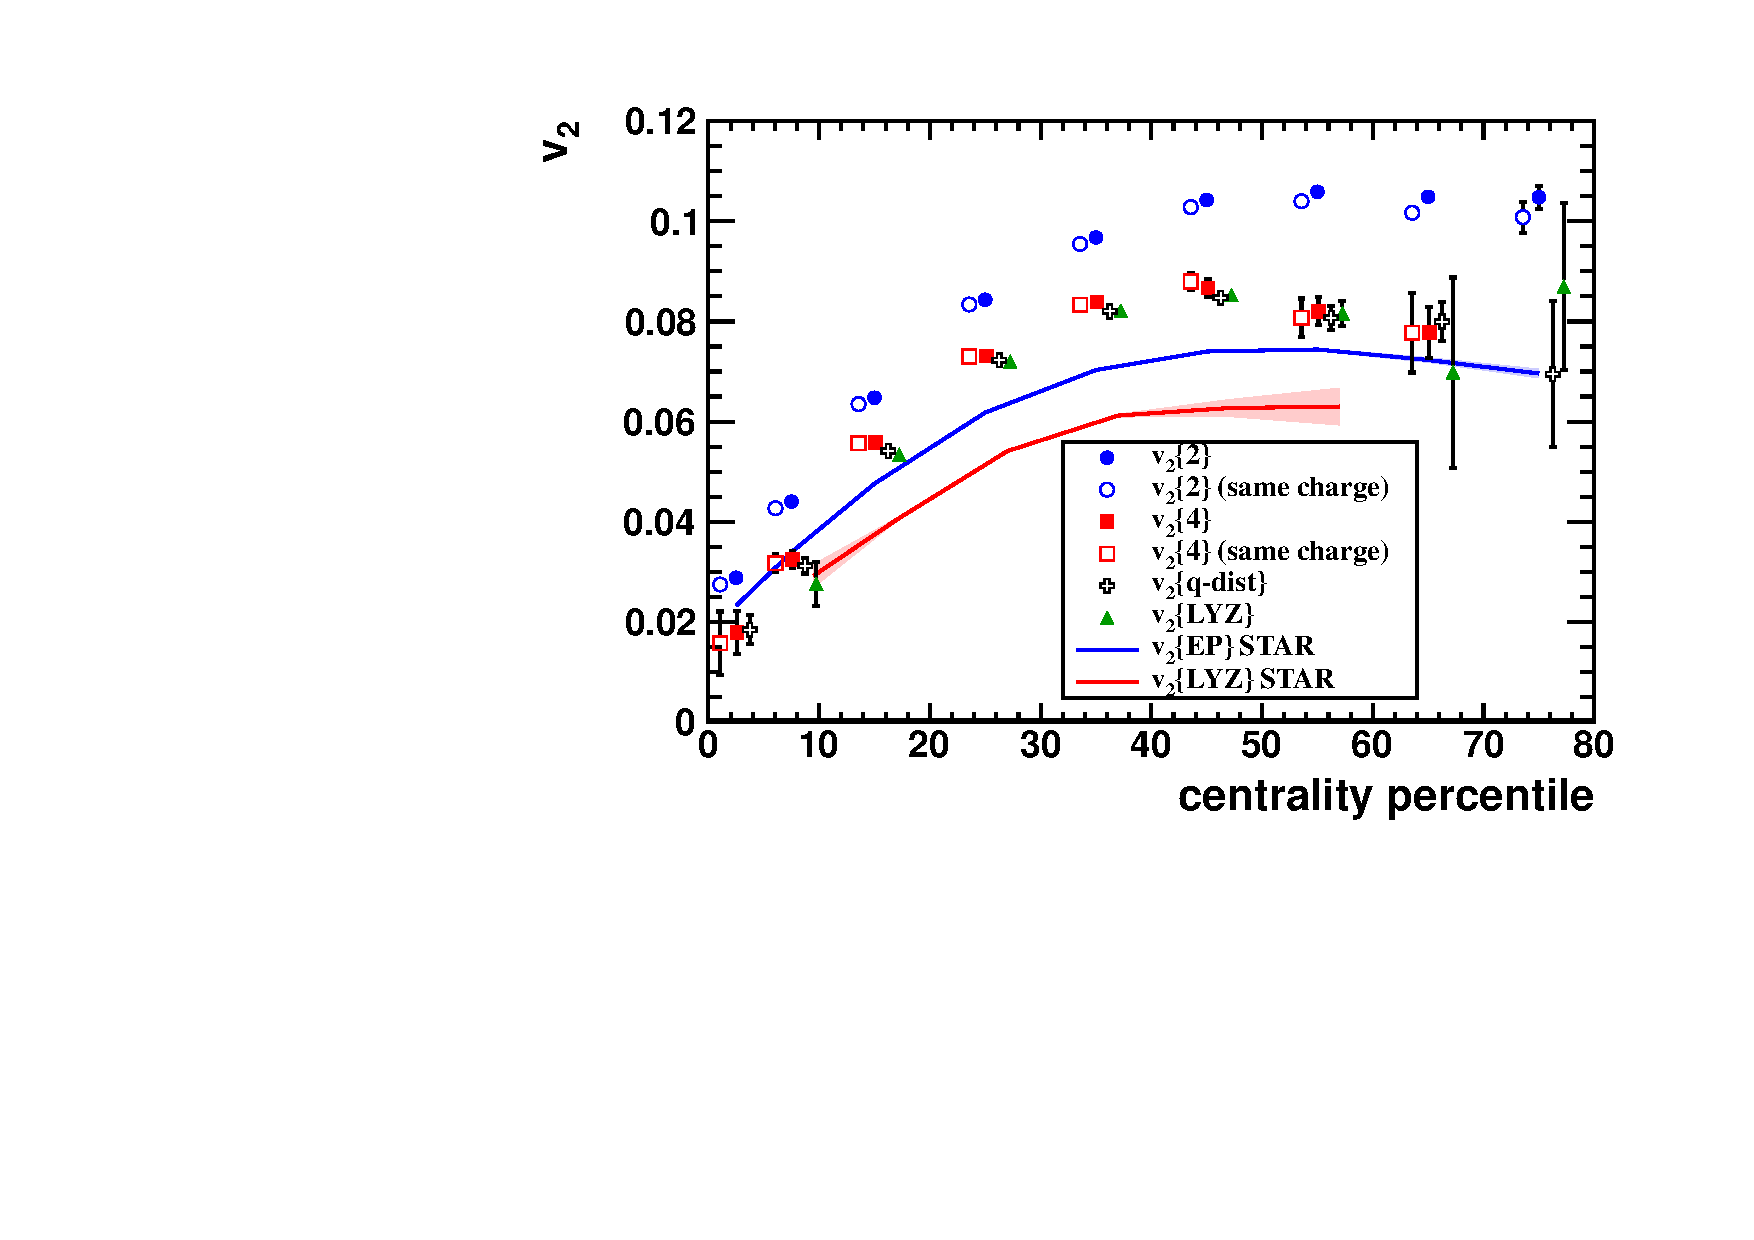
\includegraphics[width=12.0cm]{figures/alice_flow_result}}
\caption{ The published results of flow with ALICE Pb + Pb $\sqrt{S_{NN}}=2.76$~TeV with various methods \cite{Aamodt:2010pa}.} 
\label{fig:alice_flow_result}
\end{figure}


The higher-order cumulants like 6-particle or 8-particle correlation can be calculated in the same way.

\section{Jet quenching}


In $p$-$p$ collisions, hard scattered partons fragment into hadrons with high transverse momentum, also called as jets. However in heavy-ion collisions, the hard scattering occurs before the formation of QGP, and the scattered partons will experience the entire evolution of the system created in these collisions \cite{Enterria:2009am}.
These partons will interact strongly with the created medium and loss their energy, and these features are known as ``jet quenching''  \cite{PhysRevLett.68.1480}. This ``jet quenching" is the another strong evidence of the existence of the QGP, because energy loss in a deconfined matter is believed to be much stronger than in hadronic matter \cite{PhysRevLett.68.1480}. ``Jet quenching" is usually observed with the suppression of high $p_T$ particles yields though the nuclear modification factor $R_{AA}$, defined as like 
 
 \begin{equation}
	R_{AA}(p_{\rm{T}}) = \frac{dN_{ch}^{AA}(p_{\rm{T}})/dp_{\rm{T}}}{\langle N_{coll} \rangle dN_{ch}^{pp}(p_T)/dp_T}
\end{equation}

where AA denotes heavy-ion collisions and $pp$ for the $p$-$p$ collisions. the $dN_{ch}(dp_{\rm{T}})$ refer the number of charged particle produced in each collisions as a function of transverse momentum. The number of binary collisions $N_{coll}$ has been used to compare the yield of charged particle produced in AA and $p$-$p$ collisions as scaling factor. This $N_{coll}$ were calculated by Glauber model, which provide a proper normalization for a given AA centrality. 
  If there are not any medium effects on AA collisions, the heavy-ion collision can be regarded as a just simple superposition of nucleon-nucleon collisions (as like $p$-$p$) and nuclear modification factor $R_{AA}$ will be unity. Otherwise, any deviation from unity of $R_{AA}$  will indicate a certain medium effect of heavy ion collisions. 
  

\begin{figure}[!t]
\centerline{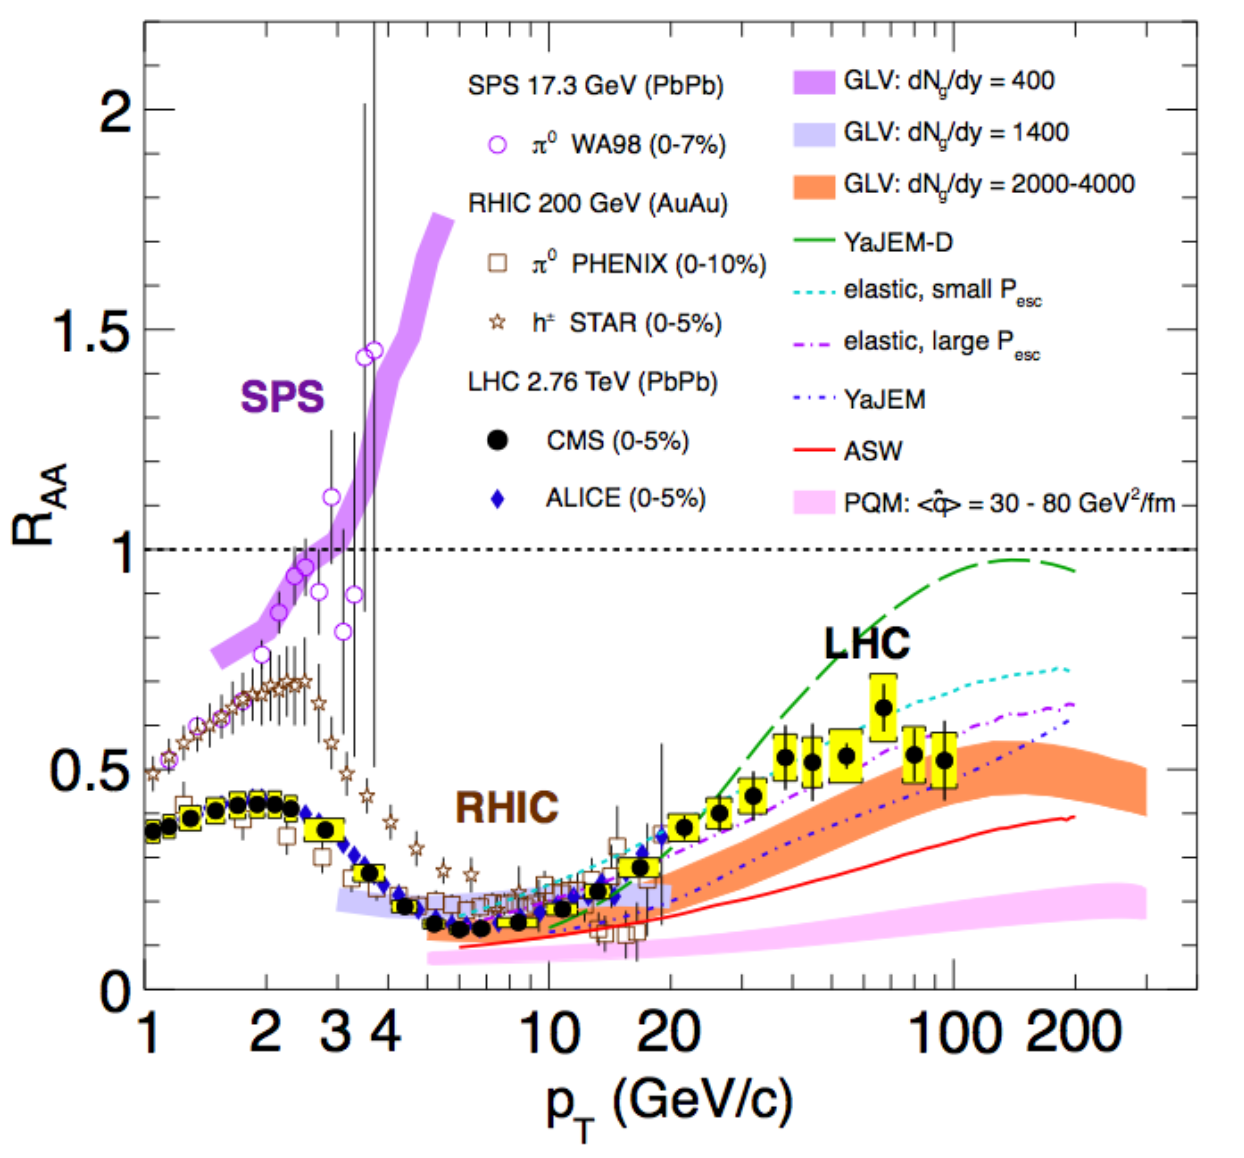
\includegraphics[width=12.0cm]{figures/raa}}
\caption{ Transverse momentum dependence of nuclear modification factor $R_{AA}$ for charged particles produced in heavy ion collisions at SPS, RHIC, and LHC \cite{Roland201470}.} 
\label{fig:RAA}
\end{figure}

    At the energy of SPS, the $R_{AA}$ was slightly lower than unity for $2 < p_T < 3$~GeV/$c$ and almost unity for above $p_T$ \cite{Aggarwaletal.2002}.   However, at RHIC energy, $R_{AA}$ increase monotonically up to $p_T \sim 3$~GeV/$c$ and then start to decrease. Hadron production for $6 < p_T < 8$~GeV/$c$ is suppressed by a factor of 5 in central Au-Au collision when compare to p-p collisions \cite{PhysRevLett.101.232301, PhysRevLett.91.172302}.
    
   Also, at ALICE energy, $R_{AA}$ published in 2010 with the $p_T$ spectra up to 20 GeV/$c$ shows a slightly stronger suppression (about a factor of 7 observed for the $p_T$ range around 6$\sim$8~GeV/$c$) than previous results was reported.  This observation was confirmed by CMS Collaborations, which extended to $p_T$ range up to 100~GeV/$c$. The $R_{AA}$ measurements exhibit a clear increasing trend up to $p_T \sim 40$~GeV/$c$ and then seems to saturate with a value of about 0.5. 
   
   
    In addition, the parton energy loss in created medium is increase as the path-length. The path-length which hard scattered parton travels are related to local geometry of create medium. Since in non-central collision the shape of collision regions are formed as like ellipse, the path-length will depend on the azimuthal angles respect to reaction plane angle. For instance, the parton travels along the minor-axis direction (in plane direction) have shorter path-length than the parton emit to the direction of major-axis (out of plane direction). As the results, at high $p_T$, $v_2$ is expected to be due to ``jet quenching'' reflecting the azimuthal asymmetry of the path-length \cite{Christiansen:2016uaq}.
    
    The study of jet energy loss in created medium as function of path-length are performed by utilizing $R_{AA}(p_{\rm{T}})$ and $v_2(p_{\rm{T}})$.  The path-length as the function of centrality and azimuthal angle respected to 2nd event plane ($\sim$ reaction plane) were estimated from Glauber simulation and details can be found in Appendix C.    
    
    
\clearpage
\section{Correlation between flow harmonics}

 Since the early 1990s the second order flow$(v_2)$ was studied as one of the most interesting results at RHIC, with Au+Au $\sqrt{S_{NN}}=200$ GeV collisions. This large signal of  the second order ``elliptic flow" are explained by the almond shape of the collision overlap region in initial state, and it indicated that a perfect liquid had been made in the early stage of collision. Also detailed studies about flow study report that the fluctuation over event-by-event leads odd number harmonics flow. 
 
 The anisotropic flow is understood as hydrodynamic response to spatial deformation of the initial density profile.
This profile fluctuates event to event due to quantum fluctuations of the positions of the constituents inside the colliding nuclei, which implies that the flow also fluctuates~\cite{Miller:2003kd,Alver:2006wh}.
The recognition of the importance of flow fluctuation has led to triangular flow and higher harmonics~\cite{Alver:2010gr,ALICE:2011ab} as well as the correlations between different Fourier harmonics~\cite{Aad:2014fla}.
 As the result from ATLAS experiments, it shows that higher order harmonics are sensitive to the $\eta/s$~\cite{Luzum:2012wu}.
And the $v_{n}$ distributions carry detailed information about the initial density profile~\cite{Renk:2014jja,Yan:2014nsa}.

However, difficulties on extracting the shear viscosity in heavy ion has been realized since it strongly depends on the specific choice of the initial conditions~\cite{Romatschke:2007mq,Luzum:2012wu,Shen:2011zc}.
The viscous effects reduce the magnitude of the elliptic flow. Furthermore, the magnitude of $\eta/s$ used in these calculations should be considered as an average over the temperature history of the expanding fireball while as it is known that $\eta/s$ of other fluids depends on temperature. 
In addition, part of the elliptic flow also can originate from the hadronic phase~\cite{Bozek:2011ua,Rose:2014fba,Ryu:2015vwa}. Therefore,
knowledge of both the temperature dependence and the relative contributions from the partonic and hadronic phases should be understood better to quantify $\eta/s$ of the partonic fluid.

The higher harmonics ($n>3$) are understood as superpositions of linear and nonlinear responses, through which they are correlated with lower-order harmonics ~\cite{Teaney:2012ke,Bravina:2013ora}. When the harmonic order is large, the nonlinear response contribution in viscous hydrodynamics is dominant~\cite{Teaney:2012ke,Bravina:2013ora}.
The magnitude of the viscous corrections as a function of $p_T$ for $v_4$ and $v_5$ are sensitive to ansatz used for the viscous distribution function, $\delta f$, a small correction for the equilibrium distribution at hadronic freeze-out when QGP phase has become cool and dilute~\cite{Luzum:2010ad}.
Hence the studies of the higher order ($n>3$) to lower order ($v_2$ or $v_3$) harmonic correlations and their $p_T$ dependence can help to understand the viscous correction to the momentum distribution at hadronic freeze-out which is probably the least understood part of hydrodynamic calculations~\cite{Teaney:2012ke,Niemi:2015qia}.


 Although there have been detailed studies of single flow harmonics in recent decades, only a few studies discussed correlation between two different flow harmonics. The difficult part of studying flow correlation is that there are two kinds of correlation between flows: the correlation between two flow magnitudes $(v_n - v_m)$, and the correlation between two flow directions. i.e., event plane angles correlation for two different flow harmonics ($\psi_n - \psi_m$).
 
 ATLAS Collaboration measured the correlation between different order event plane angles with two plane or three correlators by using two (three) subevents symmetric around $\eta = 0$ with a gap in between. With this method, we can expect the same resolution for each subevent groups and it provides its own estimate of the event plane (Fig.\ref{fig:atlas}). As a result they found a positive correlation between event plane angles as a function of centrality.
 
 CMS Collaboration also reported the correlation between different order event plane angles by using event plane methods \cite{Chatrchyan:2013kba}, which measure higher-order flow (like $v4, v5, v6$) with its own event plane angle, and also with the event plane angle which are measured from lower harmonics. For example, Fig.\ref{fig:cmsevtp} compares the $v_4$ with its own event plane angle $\Psi_4$ (i.e. $v_4\{\Psi_4\}$) and $v_4$ with 2nd order flow event plane angle $\Psi_2$ (i.e. $v_4\{ \Psi_2 \}$). 

\begin{figure}[h]
\centerline{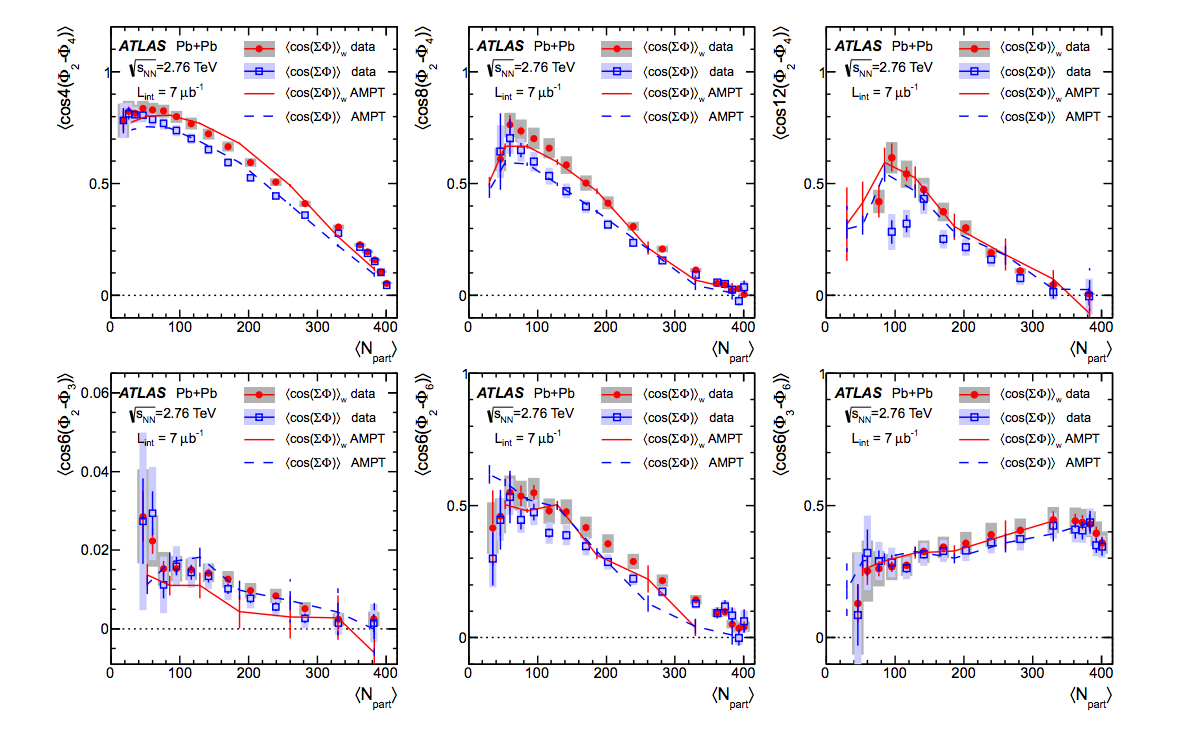
\includegraphics[width=12.0cm]{figures/atlas_eventcorr}}
\caption{ The two event plane correlators by using two subevent groups by ATLAS collaboration. $\langle \sum \Phi \rangle \equiv \langle jk(\Phi_n - \Phi_m) \rangle$.  Results from the AMPT model calculation via the SP method(solid line) and the EP method(dashed line) for represent for comparison \cite{Aad:2014fla}.} 
\label{fig:atlas}
\end{figure}


\begin{figure}[h]
\centerline{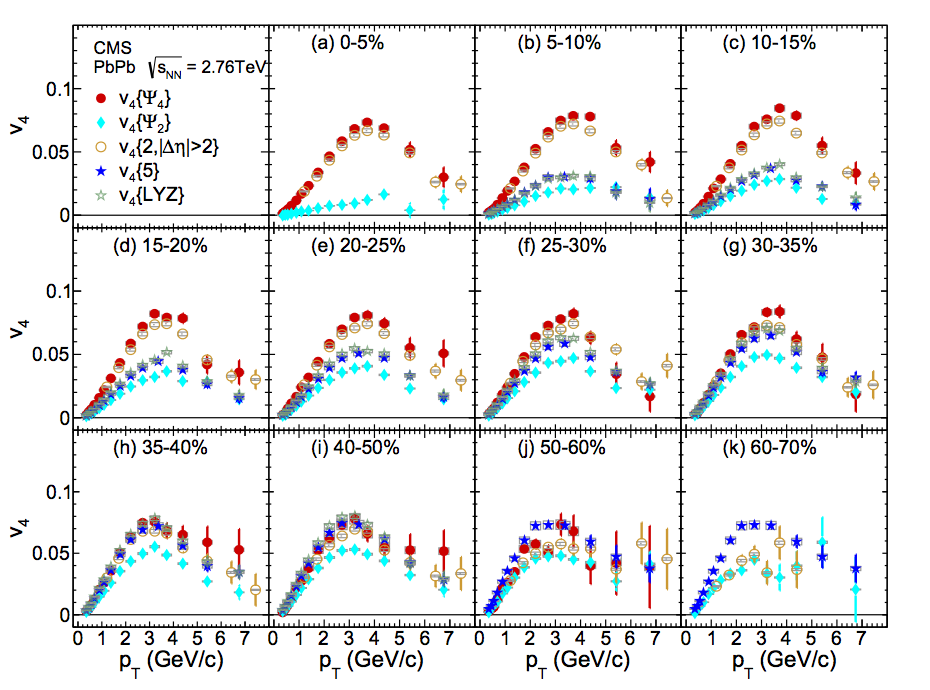
\includegraphics[width=12.0cm]{figures/cms_vn_evt}}
\caption{ Measurement of $v_4$ with different methods as a function of $p_T$ for the indicated centrality bins. The event plane method with its own event plane(red circle) and the event plane method with 2nd order event plane (blue diamonds) are drawn together.\cite{Chatrchyan:2013kba} } 
\label{fig:cmsevtp}
\end{figure}

Despite several approaches in studying flow correlations, it is still a challenge to measure only ``direction" and ``magnitudes" correlations independently. One observable proposed by H. Niemi et al. \cite{PhysRevC.87.054901} can be used to study the event-by-event fluctuations and also can measure the correlations between different $v_n$ which directly related to $\epsilon_n$. They define the linear correlation coefficients $c(a, b)$ as : 

\begin{equation}
	c(a,b) = \left\langle \frac{(a-\langle a \rangle_{ev})(b-\langle b \rangle_{ev})}{\sigma_a \sigma_b} \right \rangle_{ev}
\end{equation}
\smallskip


where $\sigma_a$ is the standard deviation of the quantity $a$. This correlation function is 1 (or -1) if $a$ and $b$ are linearly (anti-linearly) correlated and zero in the absence of correlation. From this calculation with hydrodynamic models, correlation between flow harmonics was found. The result indicates that the correlation not only depends on $\eta/s$, but is also strongly sensitive to the other properties of the QGP, such as decoupling temperature. Otherwise, the correlation $v_2$ and $v_3$ seems sensitive to the initial conditions but insensitive to $\eta/s$. Also clear $p_T$ dependence on correlation $c(v_2, v_3)$ was expected.  

Recently we measured for the first time the new multiparticle observables, the Symmetric 2-harmonic 4-particle Cumulants (SC), which quantify the relationship between event-by-event fluctuations of two different flow harmonics \cite{PhysRevC.89.064904}. The new observables are particularly robust against few-particle non-flow correlations and they provide orthogonal information to recently analysed symmetry plane correlators~\cite{ALICE:2016kpq}. 
It was demonstrated that they are sensitive to the $\eta/s$ of the expending medium and simultaneous descriptions of different order harmonic correlations would constrain 
both the initial conditions and the medium properties.
In this article, we have extended the analysis to higher order Fourier harmonic (up to 5th order) correlations as well as $p_T$ dependence of correlations for the lower order harmonic ($v_3$-$v_2$ and $v_4$-$v_2$).  We also include a systematic comparison to hydrodynamic and AMPT models.
 
   From these studies, we can understand that the flow harmonics fluctuate event-by-event due to the fluctuations in the initial matter distribution, including contributions from fluctuations in the positions of the participating nucleons in the nuclei, the participant plane, determined by the participating nucleons. In addition, such event-by-event fluctuations of the spatial asymmetry generate additional harmonics, which are more sensitive to $\eta /s$, because the effect of share viscosity reduces all anisotropic flow coefficients, with a larger decrease for higher order coefficients.  
 